\documentclass[tikz]{standalone}
\usepackage[utf8]{inputenc} 			
\usepackage[norsk]{babel}

\usepackage{amsmath, amssymb, amsthm, mathtools}   % Mijøer og verktøy for å
\usepackage{esdiff}
\let\div\relax
\DeclareMathOperator{\div}{div}
\DeclareMathOperator{\curl}{curl}
\DeclareMathOperator{\grad}{grad}
    
\newcommand{\vek}[1]{\mathbf{#1}}
\newcommand*{\dd}{\mathop{}\!{\operator@font d}}
\newcommand{\F}{\vek{F}}
\newcommand{\G}{\vek{G}}
\newcommand{\rr}{\vek{r}}
\newcommand{\dr}{\mathop{}\! \mathrm{d} \vek{r}\mathop{}\! }
\newcommand{\dt}{\mathop{}\! \mathrm{d} \vek{t}\mathop{}\! }
\newcommand{\dSS}{\mathop{}\! \mathrm{d} \vek{S}\mathop{}\! }
\newcommand{\dV}{\mathop{}\! \mathrm{d} V\mathop{}\! }

\newcommand{\R}{\mathbb{R}}

\usetikzlibrary{shapes.geometric, arrows}

\tikzstyle{startstop} = [rectangle, rounded corners, minimum width=3cm, minimum
height=1cm,text centered, draw=black, fill=red!30]
\tikzstyle{starting} = [trapezium, trapezium left angle=70, trapezium right
angle=110, rounded corners, minimum width=1cm, minimum
height=1cm,text centered, draw=black, fill=blue!40]
\tikzstyle{io} = [trapezium,
trapezium left angle=70, trapezium right angle=110, minimum width=3cm, minimum
height=1cm, text centered, draw=black, fill=blue!30]
\tikzstyle{process} =
[rectangle, minimum width=3cm, minimum height=1cm, text centered, draw=black,
fill=orange!30]
\tikzstyle{decision} = [diamond, minimum width=3cm, minimum
height=1cm, text centered, draw=black, fill=green!30]


\tikzstyle{arrow} = [thick,->,>=stealth]

\begin{document}

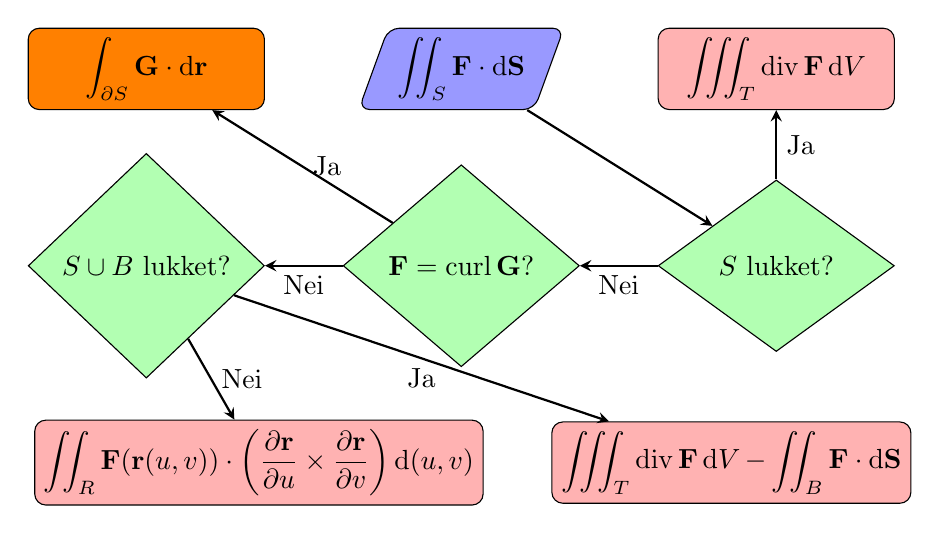
\begin{tikzpicture}[node distance=2cm]

  \node (start) [starting,fill=blue!40!white] {$\displaystyle \iint_{S} \F \cdot \dSS$};
  \node (stop1) [startstop, right of=start, xshift=2cm, align=left] {$\displaystyle\iiint_{T} \div \F \dV$};
  \node (dec1) [decision, below of=stop1, yshift=-0.5cm, align=left] {$S$ lukket?};
  \node (dec2) [decision, left of=dec1, xshift=-2cm, align=left] {$\F = \curl \G$?};
  \node (dec3) [decision, left of=dec2, xshift=-2cm, align=left] {$S \cup B$ lukket?};
  \node (stop2) [startstop, below of=dec3, yshift=-0.5cm, xshift=1.43cm, align=left] {$\displaystyle\iint_R \F(\rr(u,v))\cdot \left( \diffp{\rr}{u} \times \diffp{\rr}{v} \right)\mathrm{d}(u,v)$};
  \node (stop3) [startstop, fill=orange,above of=dec3, yshift=0.5cm, align=left] {$\displaystyle\int_{\partial S} \G \cdot \dr$};
  \node (stop4) [startstop, right of=stop2, xshift=4cm, align=left] {$\displaystyle\iiint_T \div \F \dV - \iint_B \F\cdot\dSS$};

  \draw [arrow] (start) -- (dec1);
  \draw [arrow] (dec1) -- node[anchor=west] {Ja} (stop1);
  \draw [arrow] (dec2) -- node[anchor=west] {Ja} (stop3);
  \draw [arrow] (dec3) -- node[anchor=north] {Ja} (stop4);
  \draw [arrow] (dec2) -- node[anchor=north] {Nei} (dec3);
  \draw [arrow] (dec1) -- node[anchor=north] {Nei} (dec2);
  \draw [arrow] (dec3) -- node[anchor=west] {Nei} (stop2);
\end{tikzpicture}

\end{document}